\part{Manual}

\chapter{User}

\begin{figure}[H]
	\centering
	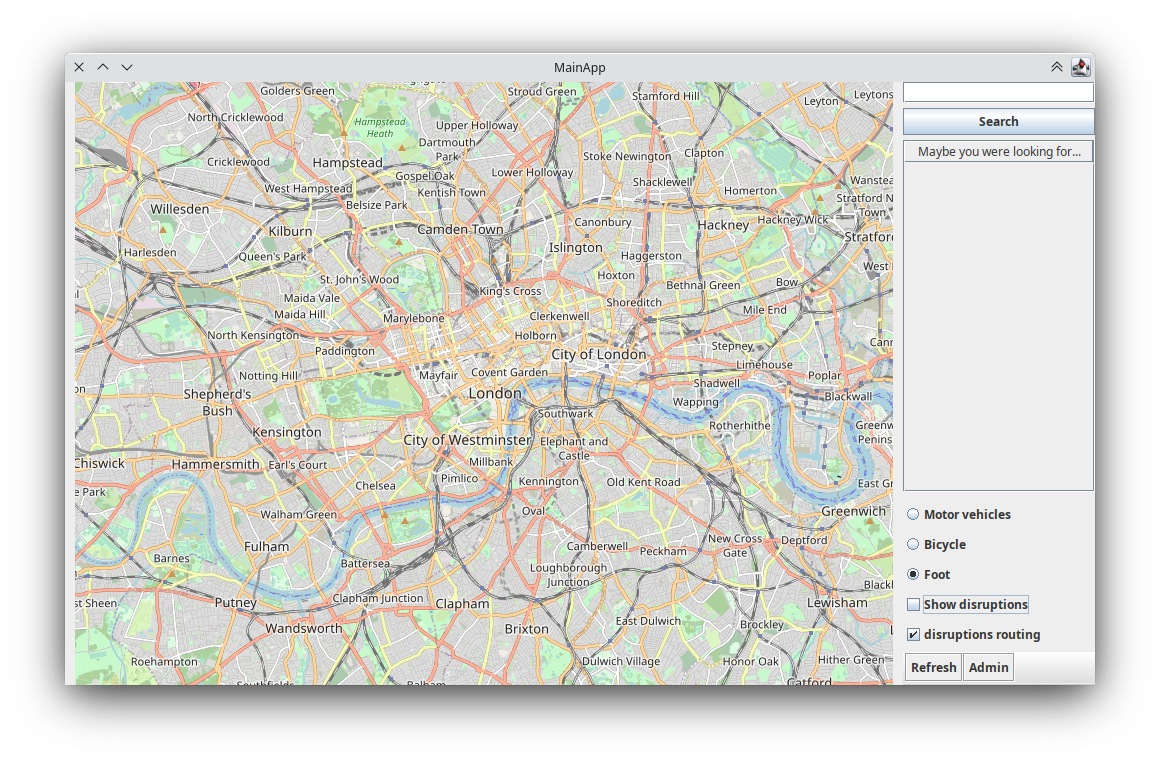
\includegraphics[width=\linewidth]{assets/mainapp0}
	\caption[]{Application just after launch}
	\label{fig:mainapp0}
\end{figure}

\paragraph{Introduction}
When launched the application automatically connects to the remote server and 
shows a map centered in London. The user can navigate the map with the typical 
\textit{drag 'n drop} that is common with those kind of applications and he can 
change the magnifying level with the scrolling wheel of the mouse.

\section{Point of interests}

\begin{figure}[H]
	\centering
	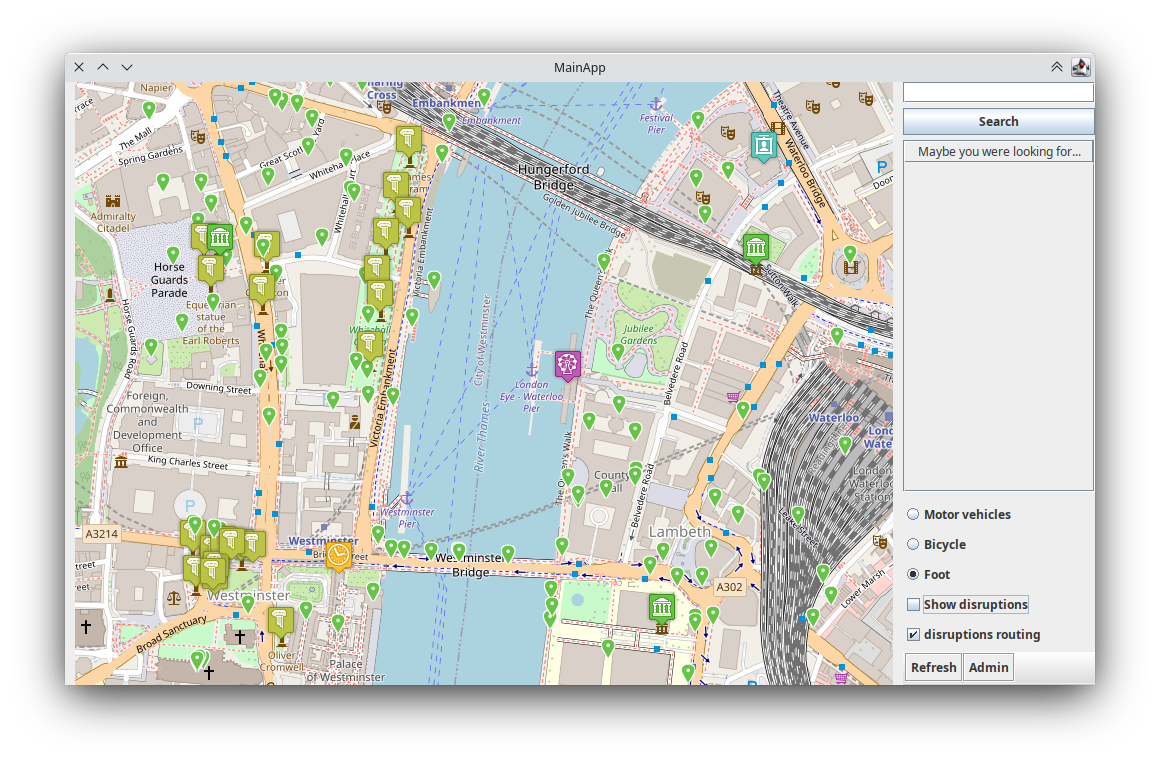
\includegraphics[width=\linewidth]{assets/mainapp1}
	\caption{Point of Interests near Westminster}
	\label{fig:mainapp1}
\end{figure}

\paragraph{Appearance}
The \textit{Point of Interest}s are being shown on the map only when an 
appropriate level of zoom is reached to avoid cluttering the map.

\paragraph{Information}
The user can access more information about a certain \textit{Point of Interest} 
by left-clicking on it. The application will then open an additional dialog 
with relevant information as seen in \ref{fig:mainappdialog1}

\begin{figure}[H]
	\centering
	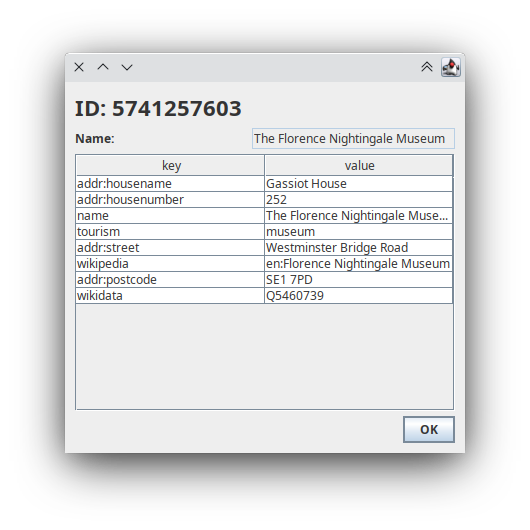
\includegraphics[width=0.5\linewidth]{assets/mainapp_dialog1}
	\caption[]{
		Informations regarding the "The Florence Nightingale Museum"
	}
	\label{fig:mainappdialog1}
\end{figure}

\section{Disruptions}

\paragraph{Appearance}
The user can make the currently active disruptions appear on the map by ticking 
the option called \textit{Show disruptions} located in the right panel. If 
needed the user can also force an update request by clicking on the button 
\textit{Refresh}.

The disruptions are color-coded according to their severity:

\begin{enumerate}
	\item \textbf{Grey} for disruptions with severity \textit{minimal}
	\item \textbf{Field drab} for disruptions with severity \textit{moderate}
	\item \textbf{Orange} for disruptions with severity \textit{serious}
	\item \textbf{Red} for disruptions with severity \textit{severe}
\end{enumerate}

\begin{figure}[H]
	\centering
	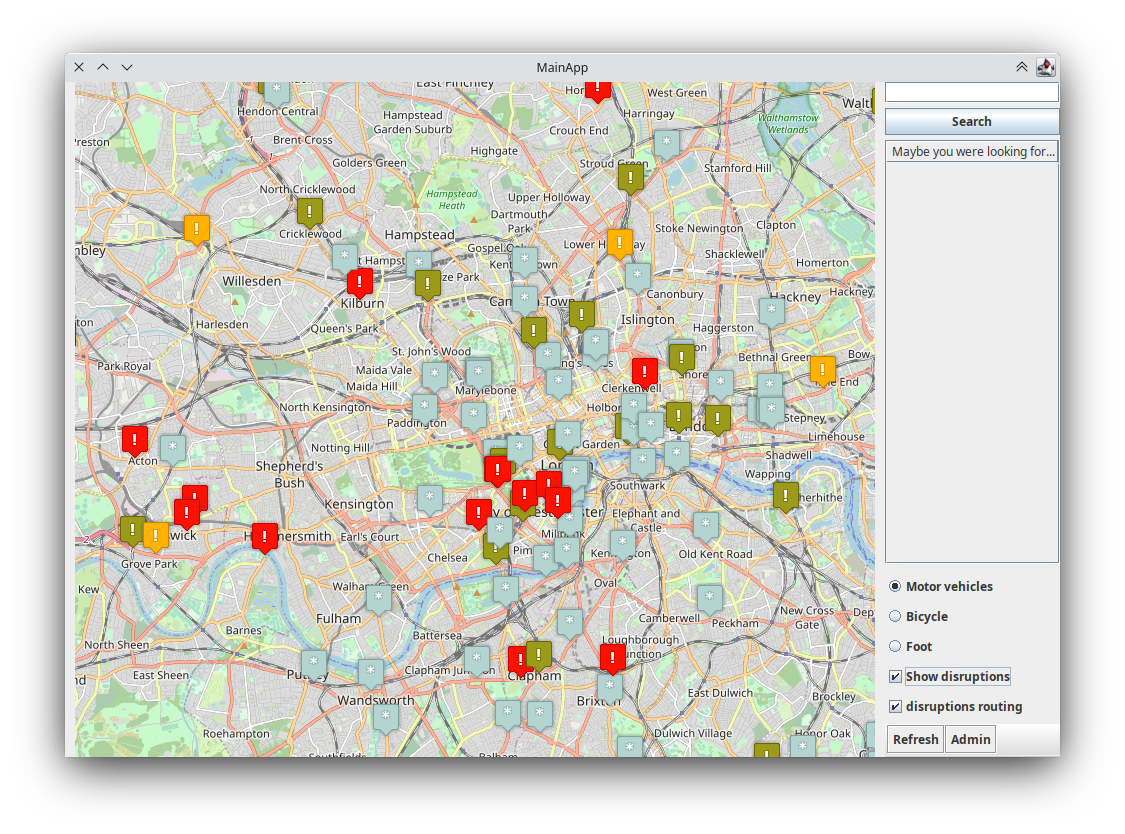
\includegraphics[width=\linewidth]{assets/mainapp2}
	\caption{Active disruptions in the afternoon of Janury 19th}
	\label{fig:mainapp2}
\end{figure}

\paragraph{Information}
The user can access more information about a certain \textit{disruption} 
by left-clicking on it. The application will then open an additional dialog 
with relevant information as seen in \ref{fig:mainappdialog2}

\begin{figure}[H]
	\centering
	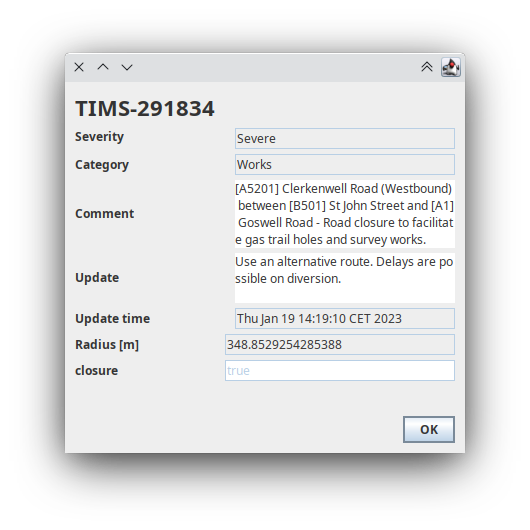
\includegraphics[width=0.5\linewidth]{assets/mainapp_dialog2.png}
	\caption[]{
		Information regarding disruption \textit{TIMS-291834}
	}
	\label{fig:mainappdialog2}
\end{figure}

\section{Routing}

\paragraph{Disruptions}
To make the routing consider delays caused by disruptions, tick the option 
called \textit{disruption routing}.

\paragraph{Mode}
The routing algorithm support three modes of transport: on foot, by bicycle or 
by car; select the appropriate option from the right panel.

\paragraph{Destination}
To route between two points, right-click on the departure point on the map then 
right click on the destination point on the map; then the routing will begin 
and the result will be rendered on the map as soon as it is available.

\begin{figure}[H]
	\centering
	\begin{subfigure}[b]{0.3\textwidth}
		\centering
		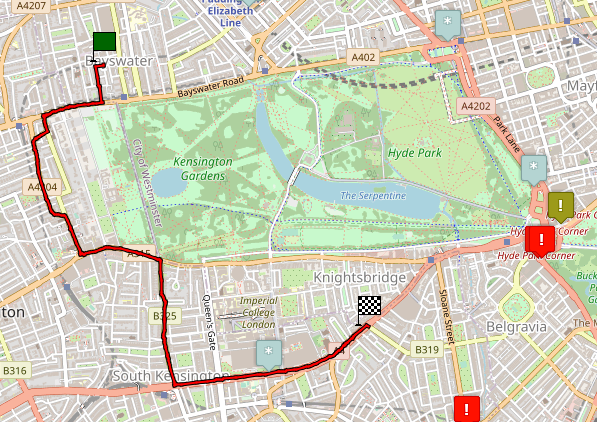
\includegraphics[width=\textwidth]{assets/routing_car.png}
		\caption{by car}
	\end{subfigure}
	\hfill
	\begin{subfigure}[b]{0.3\textwidth}
		\centering
		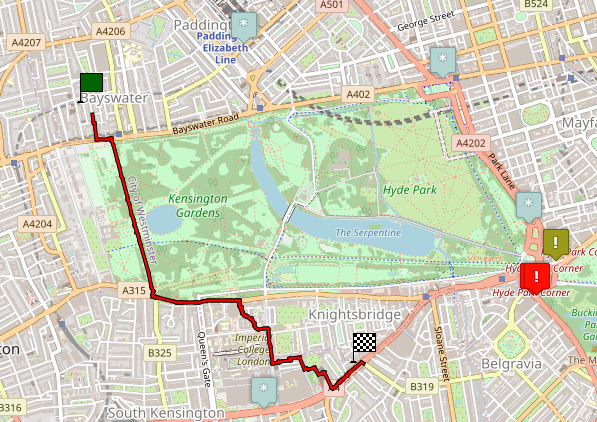
\includegraphics[width=\textwidth]{assets/routing_bike.png}
		\caption{by bicycle}
	\end{subfigure}
	\hfill
	\begin{subfigure}[b]{0.3\textwidth}
		\centering
		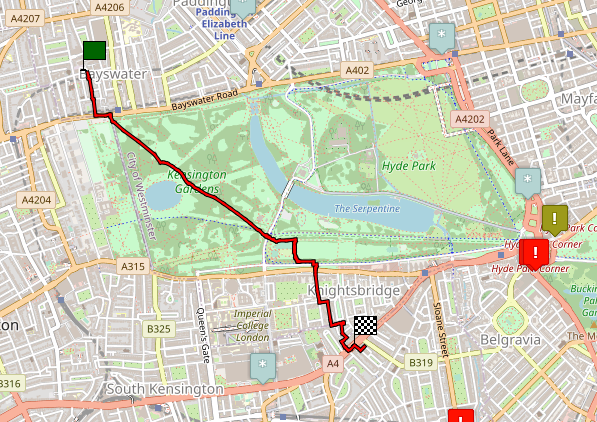
\includegraphics[width=\textwidth]{assets/routing_foot.png}
		\caption{on foot}
	\end{subfigure}
	\caption{Comparison between the three modes}
	\label{fig:routingsdiff}
\end{figure}

\paragraph{Results}
The path is rendered on the map as a red line, the estimated travel time is 
displayed in the right panel.

\begin{figure}[H]
	\centering
	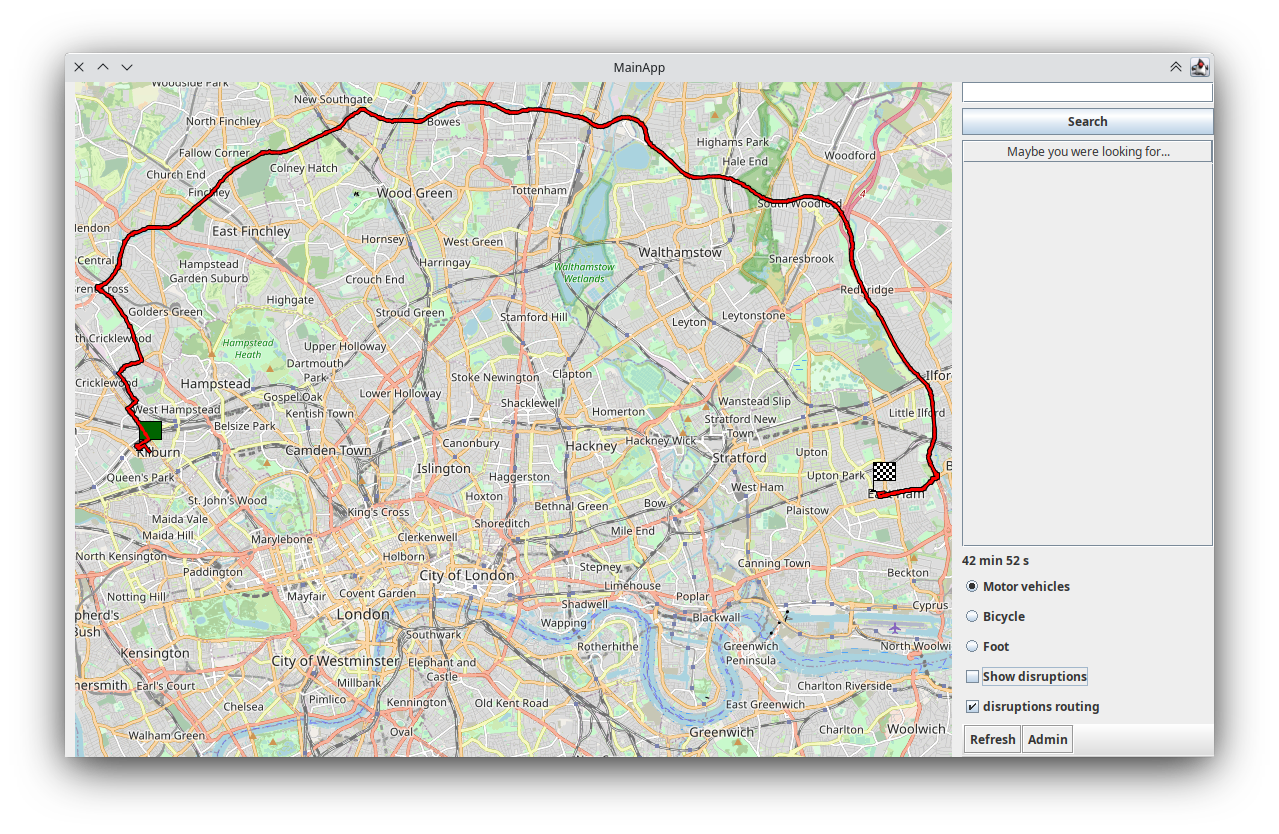
\includegraphics[width=\linewidth]{assets/mainapp3.png}
	\caption[]{
		Routing between Kilburn and East Ham.
		We can see how the routing procedure prefers faster motor-only roads 
		when traveling by car
	}
	\label{fig:mainappdialog3}
\end{figure}

\paragraph{Time estimation}
The travel time estimations considers several factors such as

\begin{itemize}
	\item The maximum speed for the given mode
	\item If in a vehicle, the speed limit
	\item If in a motor vehicle, the road class
	\item If enabled, the disruptions' severity
\end{itemize}

\begin{figure}[H]
	\centering
	\begin{subfigure}[b]{0.48\textwidth}
		\centering
		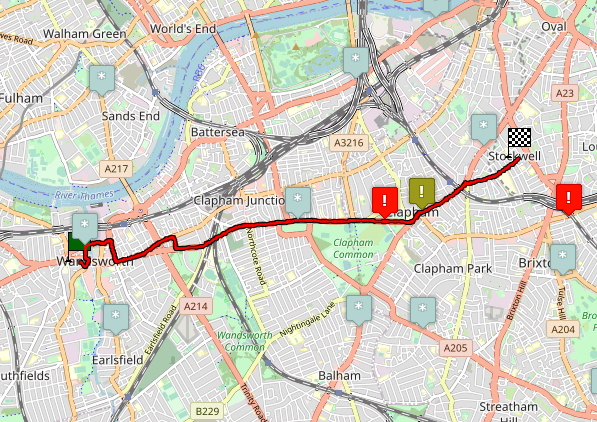
\includegraphics[width=\textwidth]{assets/routing_without_disruptions.png}
		\caption{disruptions off}
	\end{subfigure}
	\hfill
	\begin{subfigure}[b]{0.48\textwidth}
		\centering
		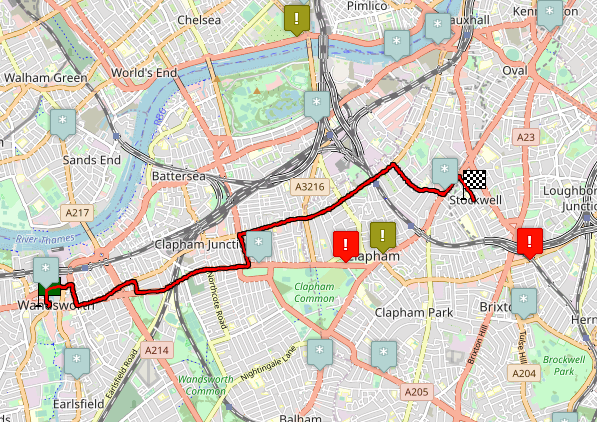
\includegraphics[width=\textwidth]{assets/routing_with_disruptions.png}
		\caption{disruptions on}
	\end{subfigure}
	\caption[]{Routing and disruptions}
\end{figure}

\pagebreak

\section{Search}

\paragraph{}
It is possible to search on the map for \textit{Point of Interest} by keyword.

\paragraph{Search}
To perform a search the user has to input his query in the\textit{Search} input 
box in the right panel and then click on the \textit{Search} button.

\paragraph{Result}
The map is centered on the most relevant \textit{Point of Interest}, other 
results are shown in a list in the right panel, below the search button.

\begin{figure}[H]
	\centering
	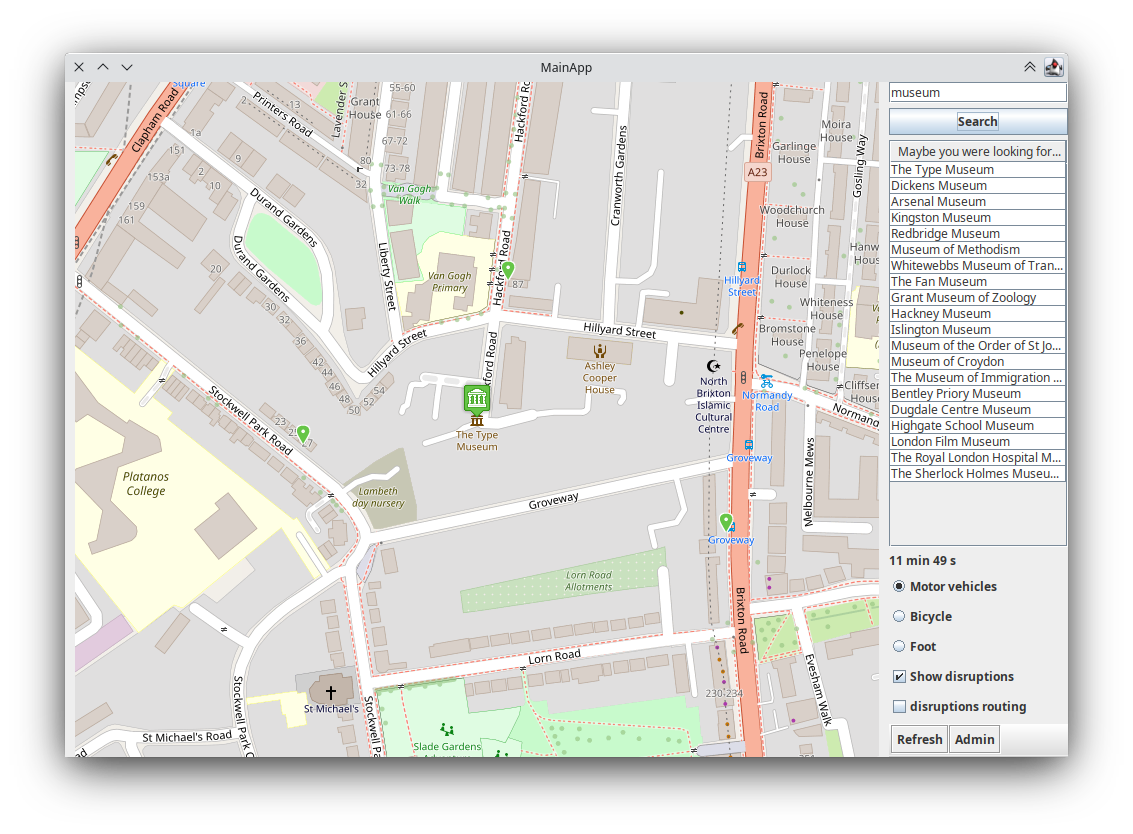
\includegraphics[width=\linewidth]{assets/mainapp4.png}
	\caption[]{
		Query results for \textit{Museum}
	}
	\label{fig:mainappdialog4}
\end{figure}

\chapter{Statistician}

\begin{figure}[H]
	\centering
	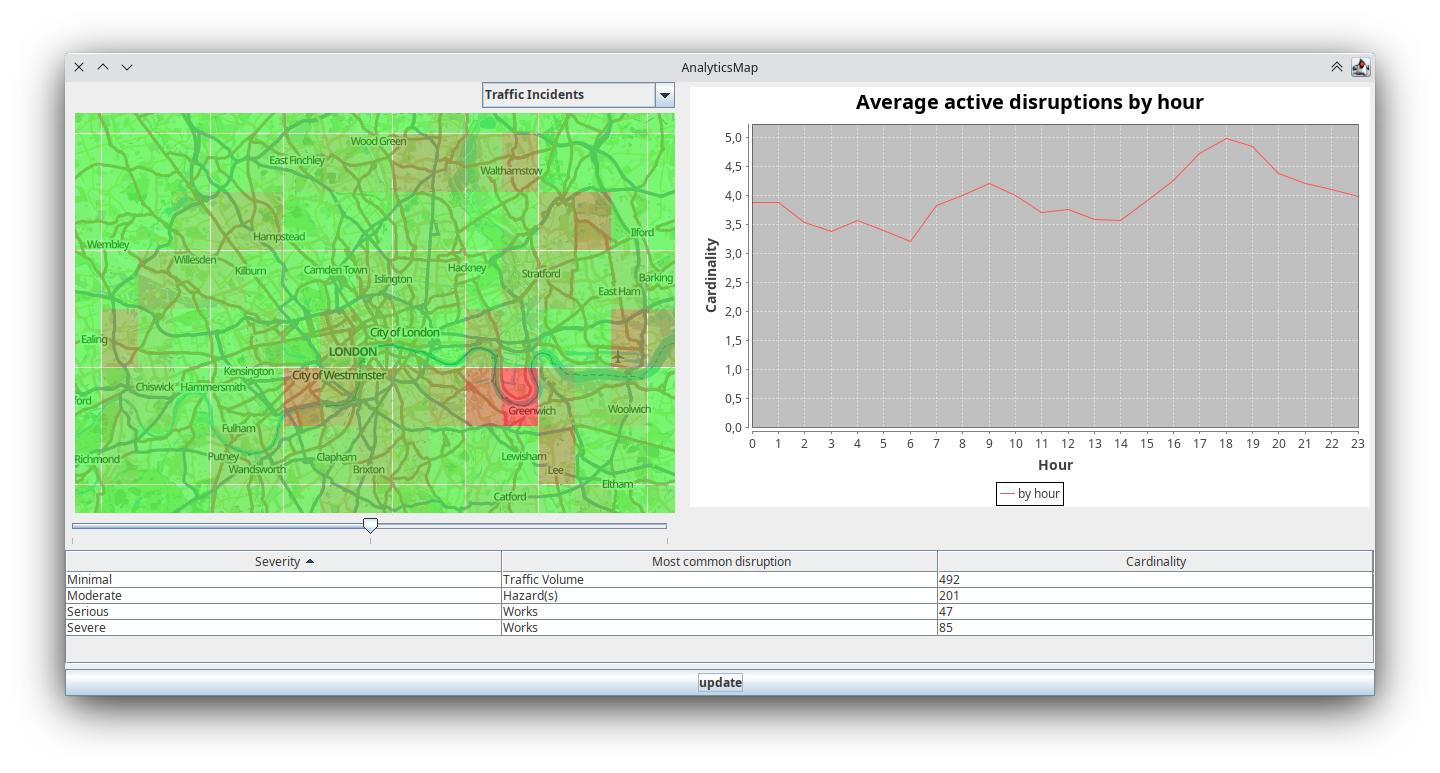
\includegraphics[width=\linewidth]{assets/anayitics0.png}
	\caption[]{}
	\label{fig:anal0}
\end{figure}

\paragraph{Access}
The authorized personnel can access the administrative window by clicking on 
the \textit{Admin} button and entering his credentials in the dialog. In the 
demo application is it possible to log-in with the following details:

\begin{lstlisting}[numbers=none, frame=single]
Username: admin
Password: admin
\end{lstlisting}

\paragraph{Layout}
The analytic window is divided in three main panels, one for each analytic 
provided by the application.

\section{Heat-map}

\paragraph{}
The heat-map is located in the top-left pane of the window. It shows a heat-map 
relative to the selected disruption; the green color represents an area where a 
the class of disruption never happened, the red color represents an area where 
most of the disruptions happened.

\paragraph{Category}
To select the \textit{category of disruption} to analyze, select it from the 
drop-down list above the map.

\paragraph{Precision}
To applications provides three levels of precision when computing the heat-map, 
to change it move the slider below the map; to the left is more precise, that 
is to render smaller squares, and to the right is less precise.

\paragraph{Movements}
As for the user's map, it is possible to move around via \textit{drag 'n drop}.

\section{Disruptions' time series}

\paragraph{}
The time series is located on the top-right pane of the window. It shows how 
common was a disruption in a certain hour of the day.

\paragraph{Category}
The category is the same as the one selected for the heat-map.

\section{Common disruptions in an area}

\paragraph{}
The result of this analytic are presented in the table located in the bottom 
pane of the window. It shows, for each category, how many disruptions happened 
in the selected area, and what was the most common sub-category for each one.

\paragraph{Boundaries}
To select the boundaries move the map around and adjust its zoom, unlike the 
others, to update the result press the \textit{update button}.  